\section{Gestione dati}
\subsection{Database}
Si � deciso di utilizzare PhpMyAdmin per la gestione del database contenente i dati del sito. 
Segue uno schema UML delle tabelle 
\begin{figure}[h]
	\centering
	\subfloat[\emph{Struttura del DB}]
	{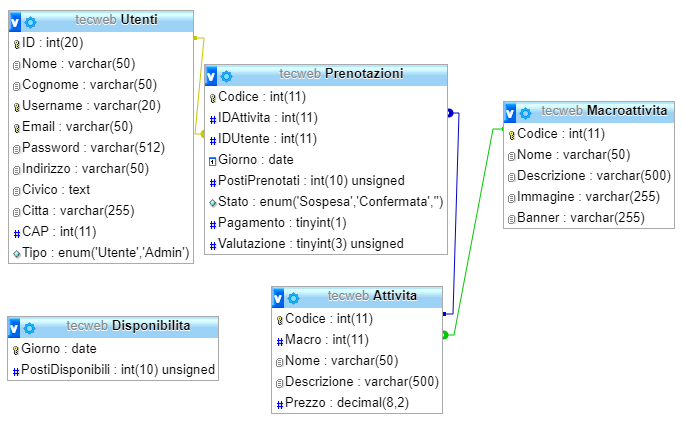
\includegraphics[scale=0.7]{images/erdb.png}}
\end{figure}
il database � inoltre privo di trigger, si � deciso infatti di gestire tramite PHP le varie operazioni riguardanti la gestione dei dati.
\subsection{Caricamento delle immagini}
Nel momento in cui viene creata una nuova macroattivit�, vi � la possibilit� di caricare  2 immagini distinte.
Tale funzionalit� � stata implementata tramite una funzione PHP uploadImage, che posiziona l'immagine nelle cartella images/attivita/index e images/attivita/banner.
Una soluzione che risulta essere in linea con il principio della dinamicit� del sito gestita, ove possibile, da PHP.